\documentclass[a4paper, 11pt]{article}
\usepackage[slovak]{babel}
\usepackage[utf8]{inputenc}
\usepackage[IL2]{fontenc}
\usepackage{times}
\usepackage{hyperref}
\hypersetup{colorlinks=true, linkcolor=black, urlcolor=blue}
\usepackage[left=1.5cm,text={18cm, 25cm},top=2.5cm]{geometry}
\usepackage{graphicx}
\graphicspath{ {images/} }
\newcommand{\myuv}[1]{\quotedblbase #1\textquotedblleft}

\begin{document}
	\sloppy
\begin{titlepage}
\begin{center}
	
	\textsc{\Huge Fakulta informačních technologií\\[3.5mm]
			Vysoké učení technické v~Brně}
	\\[79mm]
	{\LARGE IPK \,--\, Počítačové komunikace a sítě\\[1.5mm]
	Projekt č.2 - Bandwidth Measurement}
	\vfill
\end{center}
{\Large \today \hfill Tomáš Nereča(xnerec00)}
\\[-4mm]
\end{titlepage}
\tableofcontents
\thispagestyle{empty}
\newpage

\section{Zadanie}
Naštudovať problematiku merania prenosovej rýchlosti a naprogramovať aplikáciu realizujúcu meranie prenosovej rýchlosti medzi dvoma bodmi v sieti. Následne vykonať sadu experimentov pre rôzne prostredia.

\section{Základné informácie}
\subsection{Prenosová rýchlosť}
Šírka pásma by sa dala definovať ako maximálna veľkosť dát, ktoré môžu byť po sieti prenášané za určitý čas bez toho aby dochádzalo k stratám paketov. Pri \emph{UDP} komunikácii je tolerovaná stratovosť paketov 1\%. 
Existuje viacero známych prístupov merania šírky pásma. Pri svojom riešení som zvolil prístup podobný \emph{TCP} komunikácii. V prvej fáze prebieha odhad šírky pásma. Merák sa snaží posielať dáta čo najväčsou rýchlosťou. Ak prichádza k stratám väčším ako 1\%, rýchlosť odosielania sa postupne znižuje. Po odhade prebieha meranie, pričom rýchlosť sa reguluje. Ak sa pakety nestrácajú, rýchlosť sa zvyšuje a ak sa strácajú, rýchlosť sa znižuje.

\subsection{Smerodajná odchýlka \emph{(STDEV)}}
Smerodajná odchýlka udáva informácie o tom, ako široko sa rozkladajú hodnoty v množine hodnôt, t.j. k akým odchýlkam prichádza pri meraní vzhľadom k akejsi strednej hodnote - priemeru. Smerodajná odchýlka sa počíta pomocou vzorca $\sqrt{\frac{1}{N - 1} \sum\limits_{i=1}^{N} (x_i - \overline{x})^2}$, kde $N$ je počet hodnôt, $x_i$ sú jednotlivé hodnoty a $\overline{x}$ je priemer hodnôt.

\subsection{Obojsmerné oneskorenie \emph{(RTT)}}
Obojsmerné oneskorenie je doba, ktorá uplynie od odoslania paketu zadanej velkosti z jedného bodu v sieti na druhý, po príchod potvrdzujúceho paketu. Potvrdzovací paket nemá veľkosť pôvodného paketu. Je to len informácia o tom, že paket prišiel.

\section{Popis riešenia}
Po spustení aplikácie sa porovná prvý parameter s hodnotami \textsc{meter} a \textsc{reflect}. Na základe toho sa vykonáva buď funkcia \textsc{meter} alebo \textsc{reflect}. Na začiatku každej z nich sa najprv skontrolujú parametre pomocou funkcie \textsc{getopt} a v prípade správnej kombinácie parametrov následuje vytvorenie \emph{socketu} pre \emph{UDP} komunikáciu podľa postupu z prednášky.

\subsection{Merák}
Po vytvorení socketu a preklade adresy prebehne kontrola, či je \emph{port} číslo v rozsahu 0 - 65535 a veľkosť \emph{sondy} v rozsahu 64 - 64000. Ak je rozsah platný, vygeneruje sa sonda pomocou \textsc{for} cyklu. Do sondy sa vkladajú malé písmená abecedy, čo zebezpečuje delenie \emph{modulo}. Následne sa skontroluje, či je čas merania aspoň 3 sekundy a určí sa \emph{timeout} socketu a dĺžka jedného merania na základe veľkosti sondy. Štruktúra \textsc{conn} obsahuje informácie o sockete, sondu, dĺžku jedného merania, \emph{timestamp} pre dĺžku merania a RTT a príznak aktivity. Štruktúra je naplnená potrebnými hodnotami a tým pádom je všetko pripravené pre odhad rýchlosti.

Komunikácia prebieha pomocou dvoch \emph{vlákien} ktoré bežia súčasne - funkcia \textsc{sending} posiela dáta \emph{reflektoru} a funkcia \textsc{receiving} dáta prijíma. Pred odhadom rýchlosti sa vytvorí timestamp, ktorý zabezpečí, že odhad nepotrvá viac ako 30 sekúnd. Ak tento čas vyprší, aplikácia skončí s chybovou hláškou. Následne sa opakovane v cykle posielajú pakety. Dĺžka jedného merania je odmeraná pomocou timestampu, ktorý sa vytvorí pred každým meraním. Kontrola, či nebola dosiahnutá dĺžka merania, prebieha vo funkcii \textsc{receiving}. Tam sa pred každým prijatím paketu porovná aktuálny čas s timestampom pred meraním pomocou funkcie \textsc{timeInterval}, a v prípade, že bola prekročená doba merania sa nastaví príznak aktivity, ktorý zabezpečí, že funkcia \textsc{sending} prestane odosielať dáta.

Rýchlosť prenosu je riadená funkciou \textsc{usleep}, ktorá je volaná v cykle funkcie \textsc{sending}. Odhad začína s hodnotou usleep 0. Ak sa v jednom meraní stratilo viac ako 1\% paketov, je táto hodnota zvýšená o 50 (hodnoty sú v mikrosekundách). Ak sa usleep dostal na hodnotu, kedy sa straty dostanú pod 1\%, odhad rýchlosti sa ukončí.

Po odhade rýchlosti sa nastaví nový čas jedného merania a timeoutu socketu na základe parametru \textsc{time}. Meranie rýchlosti je započaté s hodnotou usleep z odhadu. Prvý odoslaný paket v každom meraní má špeciálnu hodnotu prvého bajtu a je nastavený timestamp pre RTT. Ak sa prvý prijatý paket zhoduje s touto hodnotou, je zaznamenaný uplynutý čas od timestampu pre RTT a takto sa určí hodnota RTT. Po uplynutí času merania sa vykoná výpočet rýchlosti a rýchlosť je uložená do poľa. Rýchlosť je vypočítaná ako počet prijatých paketov za dobu merania. Po vykonaní všetkých meraní sa na základe doby merania určenej užívateľom vypočíta minimálna, maximálna a priemerná hodnota zo všetkých meraní pomocou funkcií \textsc{min\_element}, \textsc{max\_element} a \textsc{accumulate}.
Smerodajná odchýlka je vypočítaná funkciou \textsc{stdev}, ktorá je implementovaná na základe vzorca pre smerodajnú odchýlku. RTT je vypočítaný ako priemer všetkých úspešných meraní RTT. Po vypísaní týchto informácií aplikácia končí.
 
\subsection{Reflektor}
Po validácii \textsc{portu} bude reflektor čakať na request. Ak príjme dáta, odošle \emph{ACK paket}, ktorý obsahuje len prvý bajt prijatého paketu. Aplikácia sa ukončí až po vyvolaní signálu pre ukončenie. Napríklad môže ísť o \emph{SIGINT} a to vstupom ctrl+c z klávesnice.


\section{Zaujímavosti}
Pri nízkej prenosovej rýchlosti a zadaní nadmernej veľkosti sondy môže trvať odhad rýchlosti dlhší čas. Ak tento čas prekročí 30s, aplikácia sa ukončí s chybovou hláškou.\\\\
Ak sa pri meraní rýchlosti nepodarí namerať RTT, na výstup sa vypíše táto informácia miesto času.\\\\
Smerodajná odchýlka sa počíta podľa varianty vzorca s N - 1, ktorá je presnejšia a keďže je zaistený minimálny počet meraní, je bezpečné použiť túto variantu.\\\\
Ak je čas merania menší ako 5 sekúnd, jednotlivé merania majú dlžku 0,5 sekundy, ak je čas menší ako 10 sekúnd, merania majú dĺžku 1 sekunda a ak je čas vyšší, merania majú dĺžku 2 sekundy.\\\\
Ak jednotlivé merania majú dĺžku 2 sekundy a zároveň čas merania nieje deliteľný 2, posledné meranie trvá 1 sekundu aby bol naplnený čas merania.\\\\
Ak užívateľ zadá čas merania 10 sekúnd, neznamená to, že časť programu kde sa merá rýchlosť pobeží 10 sekúnd. V tomto konkrétnom prípade prebehne 5 meraní dlžky 2 sekundy. Po uplynutí času 2 sekundy sa ukončí odosielanie, ale funkcia \textsc{receiving} ešte prijíma pakety, ktoré boli odoslané pred uplynutím časového limitu a skončí až keď vyprší timeout pre socket, tým sa doba behu programu predlžuje, ale reálne meranie rýchlosti trvá práve 10 sekúnd.\\\\
Hodnoty jednotlivých meraní môžu kolísať na základe zmeny hodnoty usleep.\\\\
Zmena hodnoty usleep je pri odhade vyššia ako pri meraní, aby odhad netrval príliš dlho.

\newpage
\section{Sada experimentov}
manjaro - merlin\qquad ethernet\qquad sond=512, time=4:\\
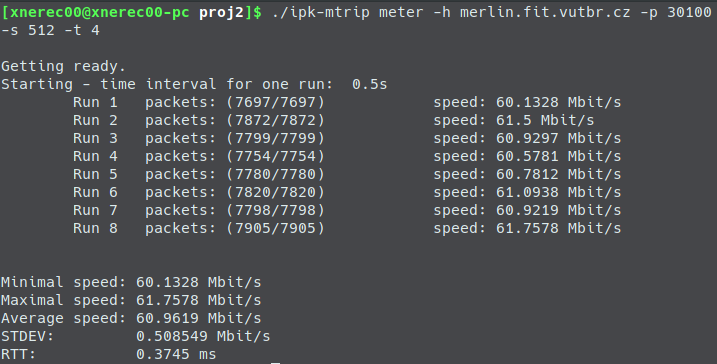
\includegraphics[scale=0.5]{pic/loc1.png}\\\\
manjaro - merlin\qquad ethernet\qquad sond=512, time=8:\\
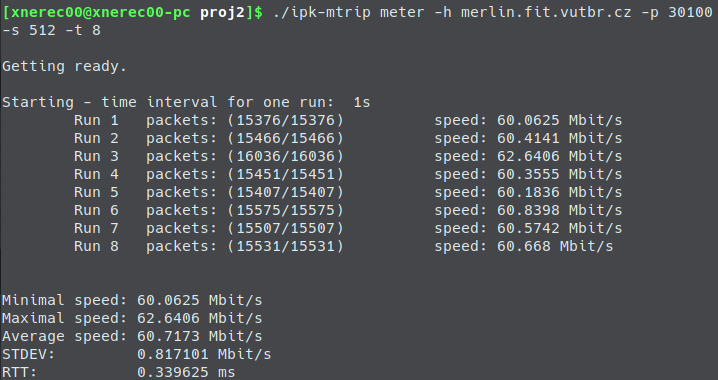
\includegraphics[scale=0.5]{pic/loc2.png}\\\\
manjaro - merlin\qquad ethernet\qquad sond=1024, time=6:\\
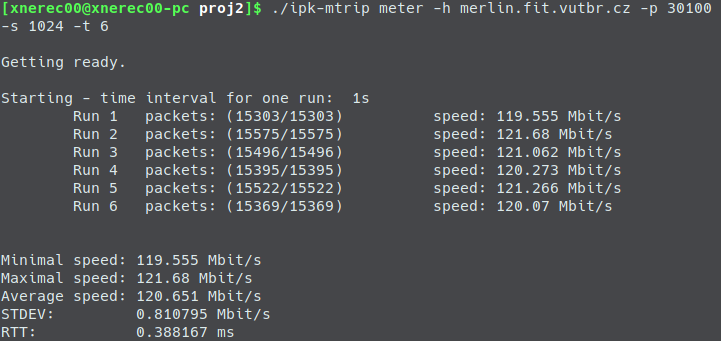
\includegraphics[scale=0.5]{pic/loc3.png}\\\\
\newpage
\noindent manjaro - merlin\qquad ethernet\qquad sond=10240, time=6:\\
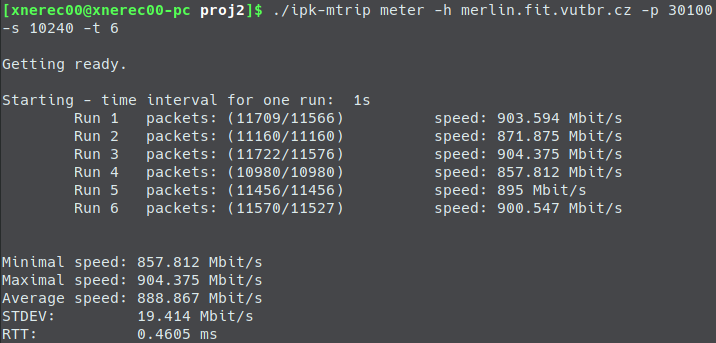
\includegraphics[scale=0.5]{pic/loc4.png}\\\\
manjaro - eva\qquad wi-fi\qquad sond=512, time=4:\\
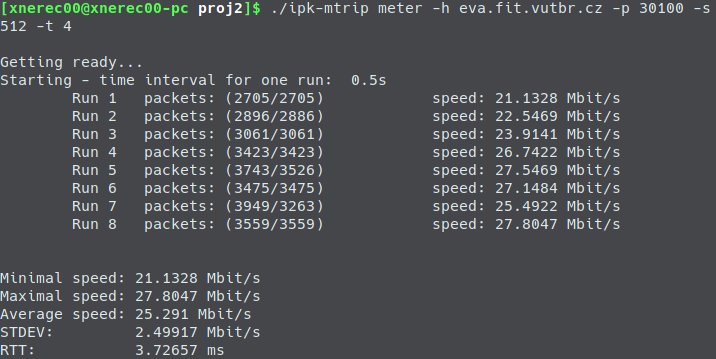
\includegraphics[scale=0.5]{pic/loc5.png}\\\\
manjaro - eva\qquad wi-fi\qquad sond=1024, time=4:\\
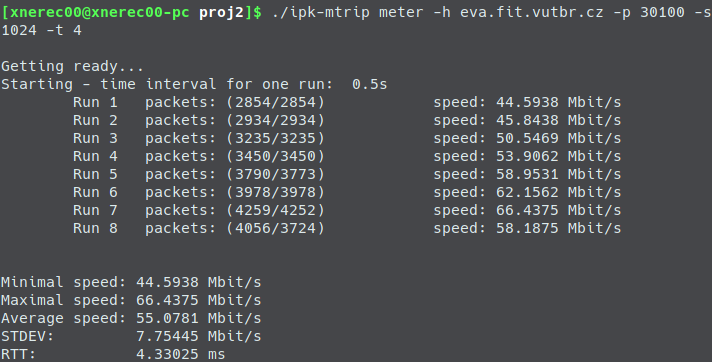
\includegraphics[scale=0.5]{pic/loc7.png}\\\\
\newpage
\noindent manjaro - eva\qquad wi-fi\qquad sond=10240, time=4:\\
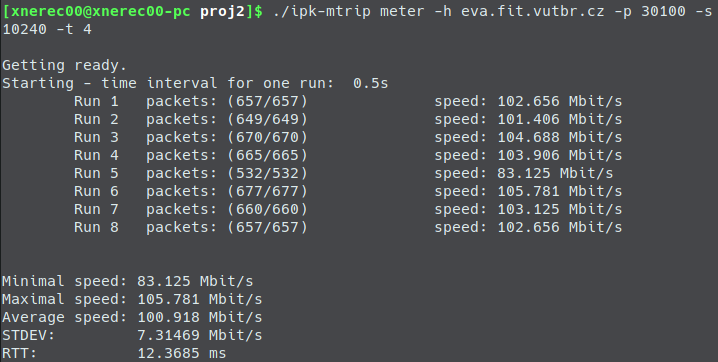
\includegraphics[scale=0.5]{pic/loc8.png}\\\\
\noindent merlin - eva\qquad sond=1024, time=4:\\
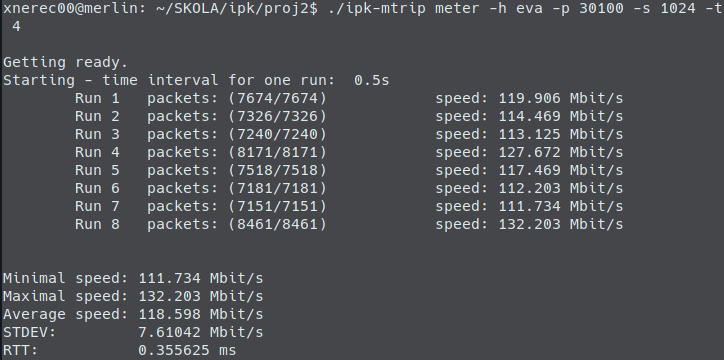
\includegraphics[scale=0.5]{pic/merlin1.png}\\\\
\noindent merlin - eva\qquad sond=10240, time=4:\\
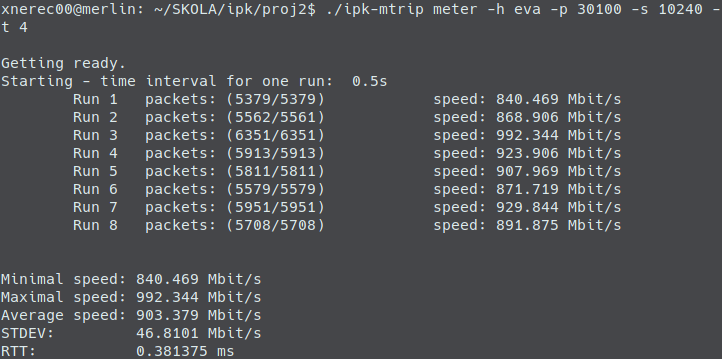
\includegraphics[scale=0.5]{pic/merlin2.png}\\\\
\newpage
\noindent eva - merlin\qquad sond=512, time=4:\\
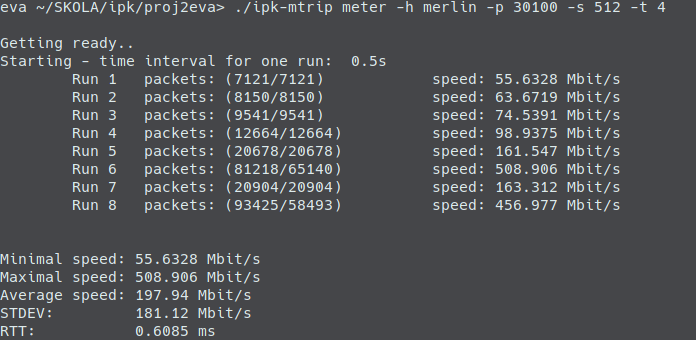
\includegraphics[scale=0.5]{pic/eva1.png}\\\\
eva - merlin\qquad sond=1024, time=4:\\
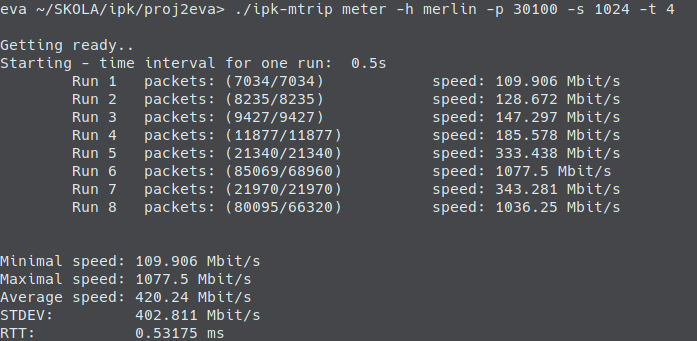
\includegraphics[scale=0.5]{pic/eva3.png}\\\\
eva - merlin\qquad sond=8000, time=4:\\
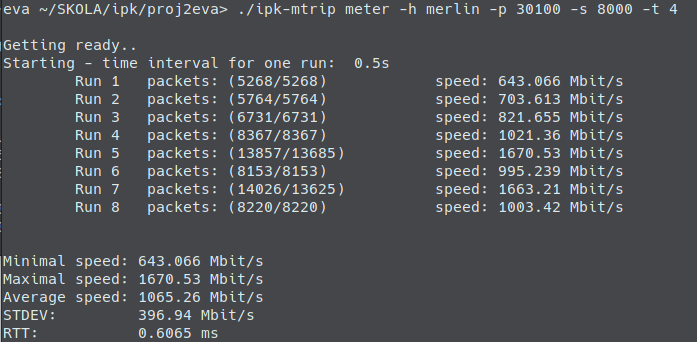
\includegraphics[scale=0.5]{pic/eva2.png}\\\\
\newpage
\noindent cent os - merlin\qquad ethernet\qquad sond=512, time=6:\\
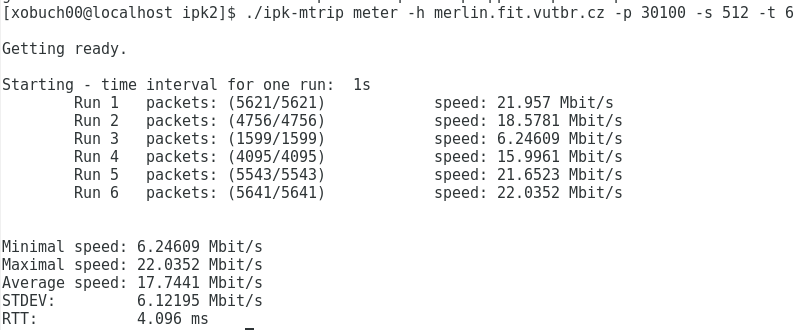
\includegraphics[scale=0.8]{pic/cent1.png}\\\\
cent os - merlin\qquad ethernet\qquad sond=1024, time=6:\\
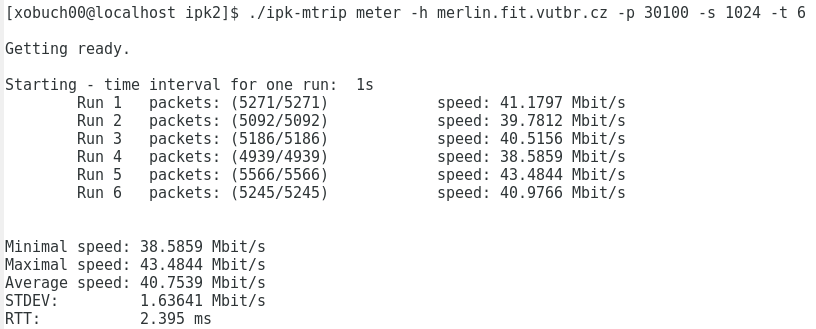
\includegraphics[scale=0.8]{pic/cent2.png}\\\\
cent os - merlin\qquad ethernet\qquad sond=10240, time=6:\\
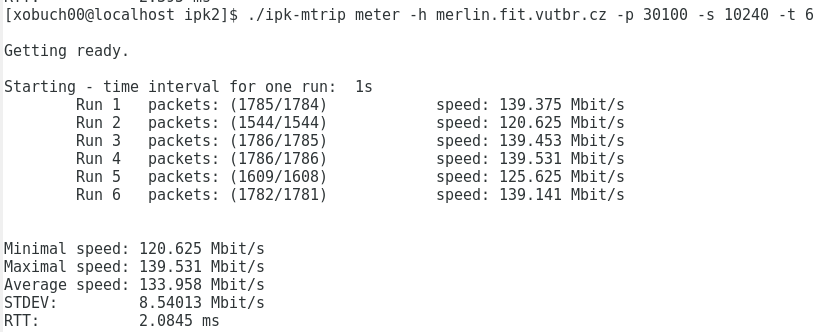
\includegraphics[scale=0.8]{pic/cent3.png}\\\\
\newpage
\noindent mac os - merlin\qquad wifi\qquad sond=512, time=6:\\
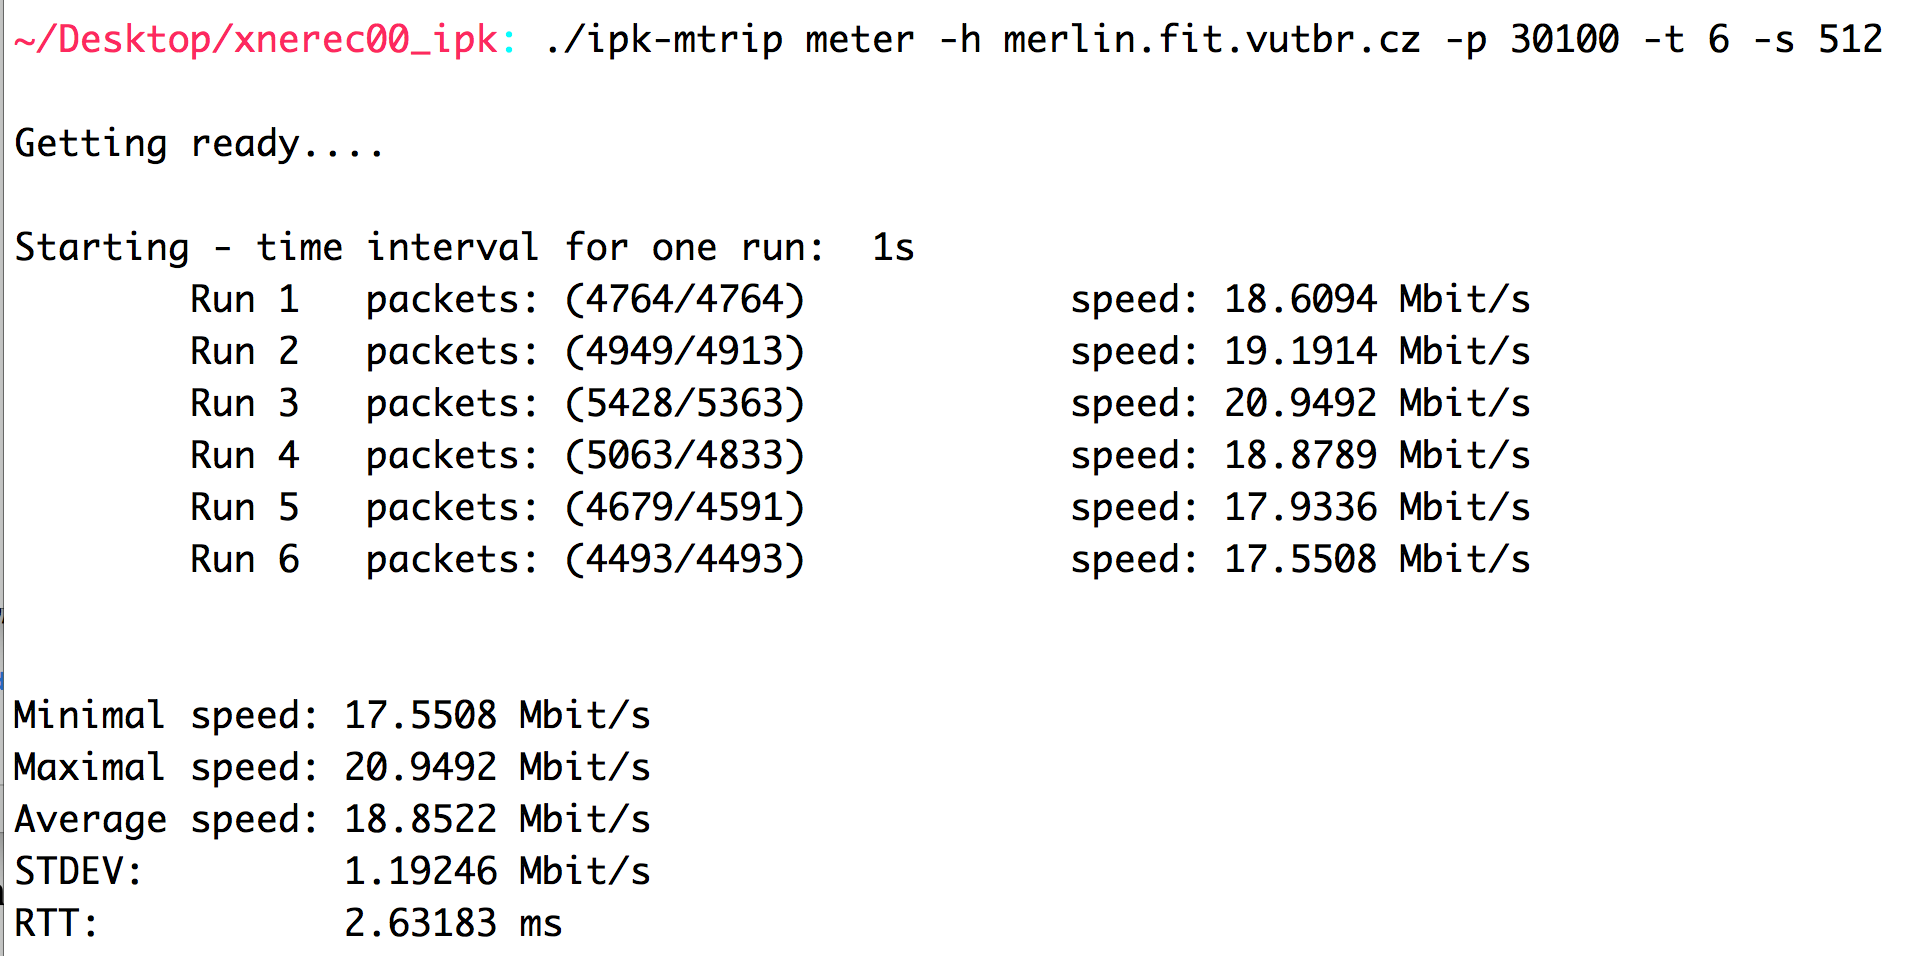
\includegraphics[scale=0.2]{pic/mac1.png}\\\\
mac os - merlin\qquad wifi\qquad sond=1024, time=6:\\
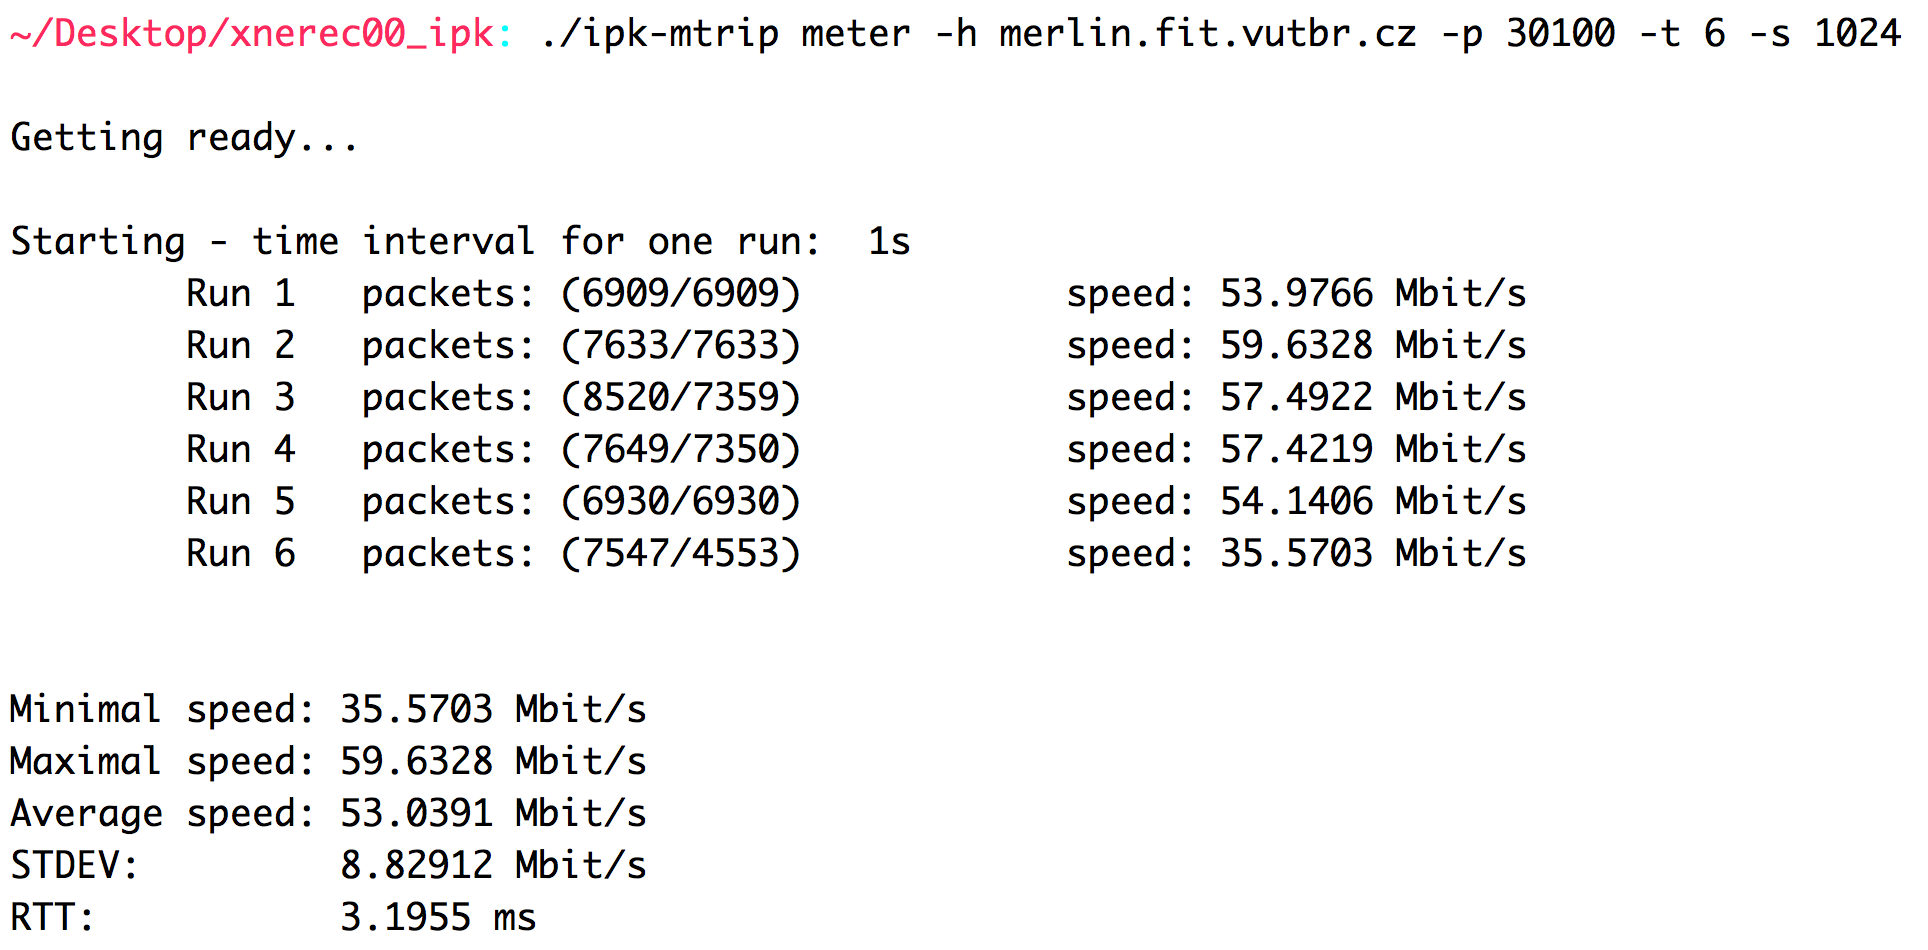
\includegraphics[scale=0.2]{pic/mac2.png}\\\\
mac os - merlin\qquad wifi\qquad sond=8000, time=6:\\
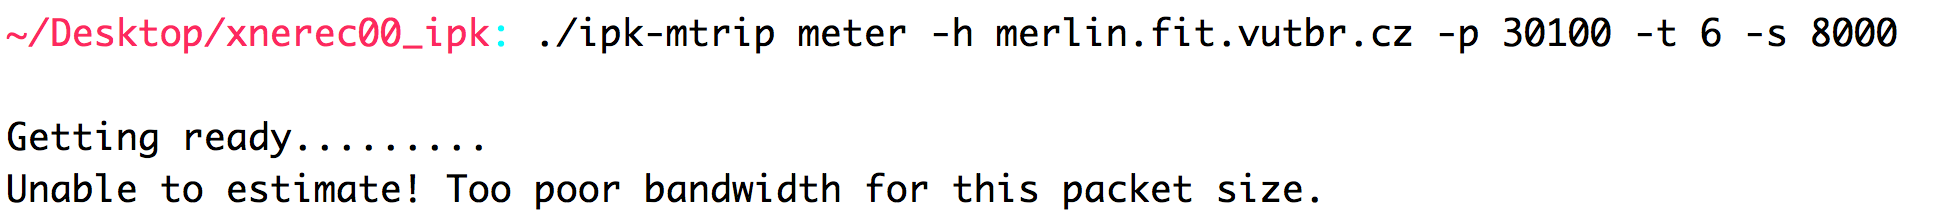
\includegraphics[scale=0.2]{pic/mac3.png}\\\\


\newpage
\section{Zdroje}
Pri návrhu UDP komunikácie som využil úryvky kódu z prednášky 2. 
Pri zisťovaní informácií o metódach merania prenosovej rýchlosti som čerpal z literatúry uvedenej v zadaní projektu, diskusných fór a wikipedie.
Ďalej som čerpal z rôznych manuálových stránok.\\\\
\url{https://www.wikipedia.org/}\\
\url{https://www.lifewire.com/what-is-bandwidth-2625809}\\
\url{https://learningnetwork.cisco.com/blogs/vip-perspectives/
	2015/10/16/bandwidth-vs-speed}\\
\url{https://stackoverflow.com/questions/3051009/c-run-two-functions-at-the-same-time}\\
\url{http://man7.org/linux/}\\
\url{https://linux.die.net/man/}\\
\url{http://www.cplusplus.com/reference/}\\

\end{document}

